% ===== Section 3: Jesus has returned ... as a piece of toast? (vision, ~24 min) =====
\topicopener{eye}{Տեսողություն}{Հիսուսը վերադարձել է... տոստի կտորի տեսքո՞վ}{Ինչ չգիտեիր տեսողական համակարգի մասին}{confused}

\begin{frame}{Ի՞նչն է ընդհանուր}
  \begin{columns}[c]
    \begin{column}{0.56\textwidth}
      {\centering
      \bigemoji[0.95cm]{bread}\ \bigemoji[0.95cm]{pizza}\ \bigemoji[0.95cm]{icecream}\ \bigemoji[0.95cm]{banana}\ \bigemoji[0.95cm]{chips}\ \bigemoji[0.95cm]{wood}\par}
      \medskip
      \begin{chatbox}
        Տոստ, տակո, պիցցա, պաղպաղակ, բանան, չիպս, լաքապատ փայտ... Ի՞նչն է ընդհանուր։ Գրիր չաթում։
      \end{chatbox}
      \onslide<2->{%
      \begin{card}[colback=butter!45!cream]
        Բոլորի վրա «տեսել են» \textbf{Հիսուսի դեմքը}։ Երբեմն՝ Մարիամ Աստվածածնի։ Կամ \textbf{Էլվիս Փրեսլիի}։ «Լուրջ, փնտրիր» (Բըրնեթ)։
      \end{card}}
    \end{column}
    \begin{column}{0.4\textwidth}
      \centering
      % A slice of toast whose burnt patches happen to make a face (pareidolia). No reveals.
\begin{tikzpicture}[scale=0.95]
  % crust and bread
  \filldraw[fill=peachdark!75!brown, draw=plum, line width=1pt]
    (-1.55,-1.7) -- (-1.55,0.75) .. controls (-2.05,1.1) and (-1.95,2.05) .. (-0.9,2.1)
    .. controls (-0.3,2.45) and (0.3,2.45) .. (0.9,2.1) .. controls (1.95,2.05) and (2.05,1.1) .. (1.55,0.75)
    -- (1.55,-1.7) -- cycle;
  \fill[butter!80!peach]
    (-1.35,-1.5) -- (-1.35,0.8) .. controls (-1.75,1.1) and (-1.7,1.85) .. (-0.85,1.88)
    .. controls (-0.3,2.2) and (0.3,2.2) .. (0.85,1.88) .. controls (1.7,1.85) and (1.75,1.1) .. (1.35,0.8)
    -- (1.35,-1.5) -- cycle;
  % toasted shading
  \fill[peachdark, opacity=0.18] (0,0.3) ellipse (1.2 and 1.5);
  % burnt patches: eyes, nose, mouth, beard
  \fill[plum!80!brown, opacity=0.55] (-0.55,0.95) ellipse (0.28 and 0.17);
  \fill[plum!80!brown, opacity=0.55] (0.55,0.95) ellipse (0.28 and 0.17);
  \fill[plum!80!brown, opacity=0.35] (-0.05,0.55) .. controls (-0.2,0.2) and (-0.15,0.0) .. (0.15,0.02) -- (0.1,0.2) -- cycle;
  \fill[plum!80!brown, opacity=0.45] (-0.5,-0.35) .. controls (-0.2,-0.55) and (0.2,-0.55) .. (0.5,-0.35)
    .. controls (0.2,-0.42) and (-0.2,-0.42) .. cycle;
  \fill[plum!80!brown, opacity=0.2] (-0.9,-0.1) .. controls (-0.8,-1.2) and (0.8,-1.2) .. (0.9,-0.1)
    .. controls (0.6,-0.85) and (-0.6,-0.85) .. cycle;
  % crumbs
  \foreach \x/\y in {-1.0/-1.1, 0.9/-0.9, 1.0/1.5, -1.1/1.55, 0.3/-1.25}{\fill[peachdark!70] (\x,\y) circle (0.04);}
\end{tikzpicture}

    \end{column}
  \end{columns}
\end{frame}

\begin{frame}{Դեմքեր ամենուր}
  \begin{columns}[c]
    \begin{column}{0.5\textwidth}
      \centering
      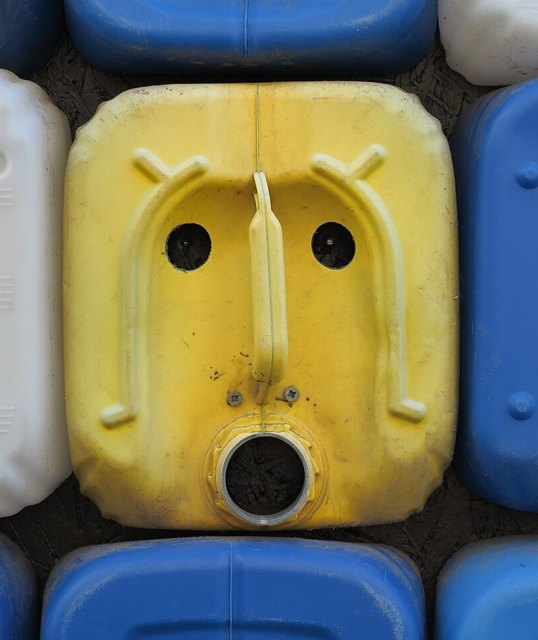
\includegraphics[height=2.45cm]{pareidolia_canister.jpg}\hspace{1mm}%
      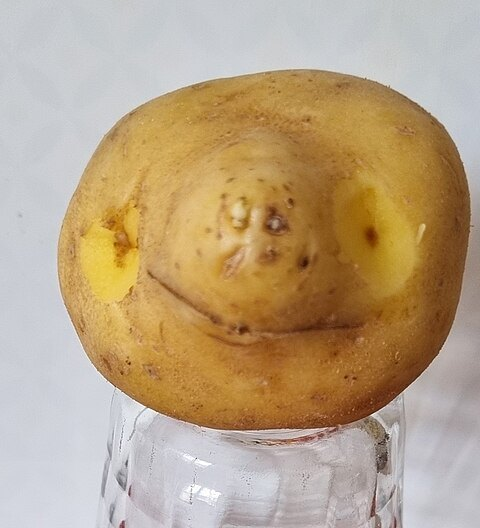
\includegraphics[height=2.45cm]{pareidolia_potato.jpg}\par\vspace{1mm}
      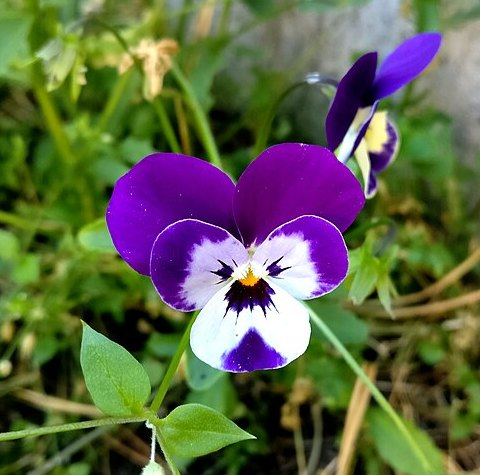
\includegraphics[height=2.45cm]{pareidolia_pansy.jpg}\hspace{1mm}%
      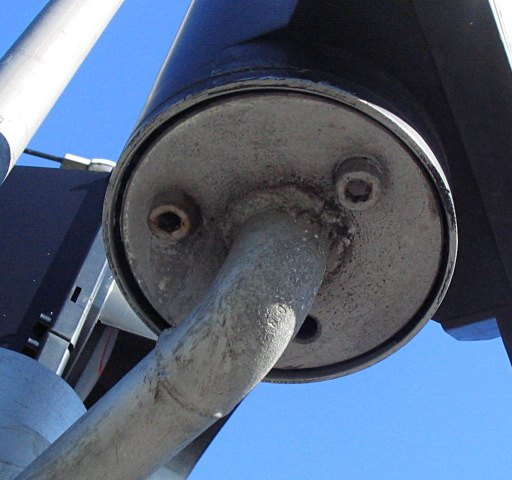
\includegraphics[height=2.45cm]{pareidolia_lamp.jpg}
    \end{column}
    \begin{column}{0.46\textwidth}
      \begin{itemize}
        \item Աշխարհում միլիարդավոր առարկաներ ունեն լուսավոր ու մուգ պատահական բծեր
        \item<2-> Պատահաբար որոշները նման են \textbf{դեմքի}։ Դա կոչվում է \textbf{պարեյդոլիա} (pareidolia)
        \item<3-> Տարօրինակն այն է, որ նույնիսկ գիտենալով, որ սա կարտոֆիլ է, դեմքը \textbf{չես կարող չտեսնել}
      \end{itemize}
    \end{column}
  \end{columns}
\end{frame}

\begin{frame}{Դեմք Մարսի վրա}
  \begin{columns}[T]
    \begin{column}{0.4\textwidth}
      \centering
      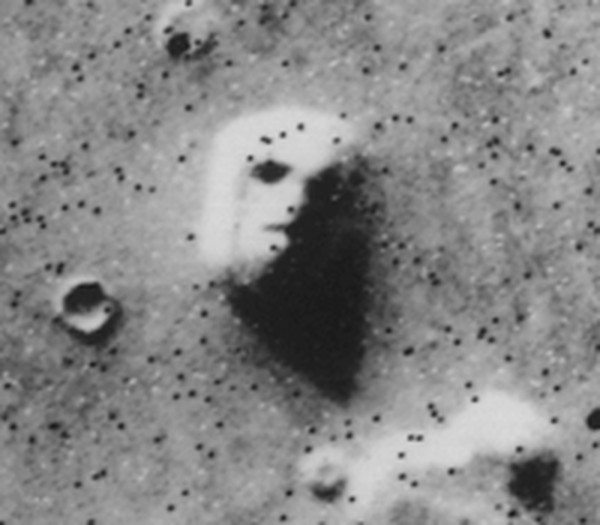
\includegraphics[height=4.1cm]{mars_face_viking_1976.jpg}\par
      {\scriptsize «Վիկինգ 1», 1976}
    \end{column}
    \begin{column}{0.56\textwidth}
      \onslide<2->{%
      \begin{columns}[T]
        \begin{column}{0.48\linewidth}
          \centering
          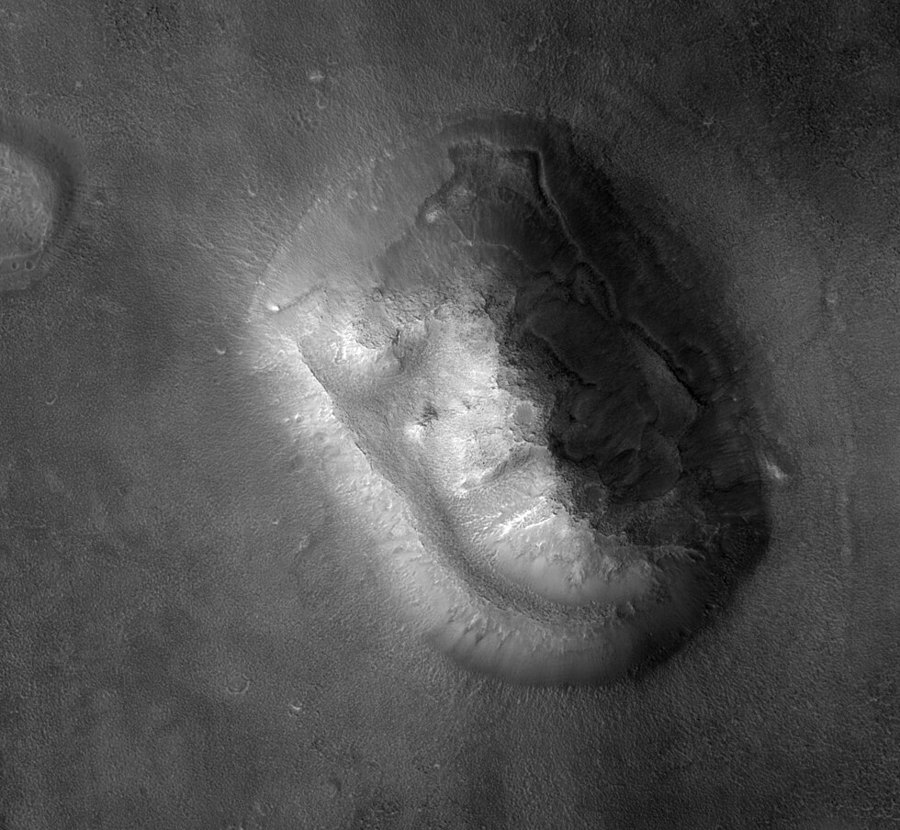
\includegraphics[height=2.9cm]{mars_face_hirise_2007.jpg}\par
          {\scriptsize Նույն բլուրը, 2007}
        \end{column}
        \begin{column}{0.5\linewidth}
          \small 1976-ին ՆԱՍԱ-ի նկարում Մարսի վրա «դեմք» երևաց։ Ավելի լավ տեսախցիկը ցույց տվեց սովորական \textbf{բլուր}։
        \end{column}
      \end{columns}}
      \vspace{2mm}
      \onslide<3->{%
      \begin{card}[colback=lavender!40!cardwhite]
        \small Ձախ նկարում դեմքը հիմա էլ տեսնում ես։ Ուղեղը դեմքեր փնտրում է \textbf{ամենուր}։
      \end{card}}
    \end{column}
  \end{columns}
  \source{NASA/JPL (Viking 1; MRO HiRISE)}
\end{frame}

\begin{frame}{Աչքերը տեսախցիկ չեն}
  \begin{columns}[T]
    \begin{column}{0.5\textwidth}
      \begin{itemize}
        \item Ուղեղը տեսողությունը գերադասում է \textbf{բոլոր} մյուս զգայարաններից
        \item<2-> Բայց աչքերը «երկու անհանգստացնող փափուկ տեսախցիկ» չեն, որոնք ամեն ինչ ուղիղ ուղեղ են փոխանցում
        \item<3-> Շատ նեյրոգիտնականներ \textbf{ցանցաթաղանթը} (retina) համարում են ուղեղի մաս. նույն հյուսվածքից է զարգանում ու ուղիղ կապված է նրան
      \end{itemize}
    \end{column}
    \begin{column}{0.46\textwidth}
      \onslide<4->{%
      \begin{bookquote}
        Աչքը այնքան բարդ է, որ այն բերում են որպես ապացույց, թե էվոլյուցիան իրական չէ։ Բայց եթե նայես, թե ինչպես է աչքը աշխատում, ստեղծողը այն նախագծել է ուրբաթ կեսօրից հետո կամ խումհարով։
      \end{bookquote}}
    \end{column}
  \end{columns}
\end{frame}

\begin{frame}{Ցուպիկներ ու սրվակներ}
  \begin{columns}[T]
    \begin{column}{0.47\textwidth}
      \begin{card}[colback=lavender!35!cardwhite]
        \tikz[baseline=-0.5ex]{\filldraw[fill=night!70, draw=plum, line width=0.6pt, rounded corners=0.6mm] (0,-0.12) rectangle (0.9,0.12);}\
        {\blackfont Ցուպիկներ} (rods)\par\smallskip
        \begin{itemize}
          \item Արձագանքում են ընդամենը \textbf{մոտ 6 ֆոտոնի}
          \item Լույս ու մութ, կոնտրաստ. աշխատում են \textbf{մթնշաղին}
          \item Ցերեկը «խեղդվում» են. մի դույլ ջուր՝ ձվի բաժակի մեջ
        \end{itemize}
      \end{card}
    \end{column}
    \begin{column}{0.47\textwidth}
      \onslide<2->{%
      \begin{card}[colback=peach!40!cardwhite]
        \tikz[baseline=-0.5ex]{\filldraw[fill=amOrange, draw=plum, line width=0.6pt] (0,-0.14) -- (0.75,-0.05) -- (0.75,0.05) -- (0,0.14) -- cycle;}\
        {\blackfont Սրվակներ} (cones)\par\smallskip
        \begin{itemize}
          \item Զգում են լույսի ալիքի երկարությունը՝ \textbf{գույնը}
          \item Ավելի մանրամասն պատկեր են տալիս
          \item Շատ լույս է պետք. դրա համար մթնշաղին գույներ չենք տեսնում
        \end{itemize}
      \end{card}}
    \end{column}
  \end{columns}
  \vspace{2mm}
  \onslide<3->{\centering\small\emoji{siren}\ Ցուպիկների զգայունությունը, ըստ Բըրնեթի, բանկի ահազանգ է, որ միանում է, երբ ինչ-որ մեկը \textbf{միայն մտածում է} կողոպուտի մասին։\par}
\end{frame}

\begin{frame}{Աչքի ներսում}
  \begin{columns}[c]
    \begin{column}{0.54\textwidth}
      \centering
      % Cross-section of the eye (light comes from the left): pupil, lens, retina, fovea, optic nerve.
% The fovea is highlighted on slide 2 (use inside a frame).
\begin{tikzpicture}[
    tagl/.style={font=\scriptsize, text=plum, align=center, inner sep=1.5pt},
  ]
  \path[use as bounding box] (-4.2,-2.25) rectangle (3.6,2.2);
  % optic nerve (behind the eyeball)
  \filldraw[fill=butter!80!cardwhite, draw=plum, line width=0.9pt]
    (1.35,-0.45) .. controls (2.2,-0.5) and (2.8,-0.75) .. (3.6,-0.95) -- (3.6,-0.25)
    .. controls (2.8,-0.05) and (2.2,0.05) .. (1.45,0.0) -- cycle;
  % eyeball and cornea
  \filldraw[fill=cardwhite, draw=plum, line width=1.1pt] (0,0) circle (1.6);
  \draw[plum, line width=1.1pt, fill=lavender!30!cardwhite] (-1.38,0.8) .. controls (-1.95,0.45) and (-1.95,-0.45) .. (-1.38,-0.8);
  % retina lining the back
  \draw[brainpink!90!plum, line width=3.2pt] (115:1.47) arc (115:-115:1.47);
  % iris with the pupil gap, lens
  \draw[amBlue!70, line width=3pt] (-1.42,0.78) -- (-1.42,0.28) (-1.42,-0.28) -- (-1.42,-0.78);
  \filldraw[fill=lavender!60!cardwhite, draw=plum, line width=0.8pt] (-1.05,0) ellipse (0.2 and 0.58);
  % light from an object, focused on the fovea
  \node at (-3.75,0.95) {\bigemoji[0.7cm]{tree}};
  \draw[amOrange, line width=0.9pt] (-3.45,0.95) -- (-1.05,0.45) -- (1.47,0.0);
  \draw[amOrange, line width=0.9pt] (-3.45,0.95) -- (-1.05,-0.4) -- (1.47,0.0);
  % fovea
  \fill[amRed] (1.47,0.0) circle (0.09);
  \begin{scope}[visible on=<2->]
    \draw[amRed, line width=1.4pt] (1.47,0) circle (0.24);
  \end{scope}
  % labels
  \node[tagl, anchor=south] at (-1.42,1.0) {բիբ};
  \draw[plum!70, line width=0.5pt] (-1.42,1.02) -- (-1.42,0.4);
  \node[tagl, anchor=north] at (-1.05,-0.95) {ոսպնյակ};
  \draw[plum!70, line width=0.5pt] (-1.05,-0.95) -- (-1.05,-0.6);
  \node[tagl, anchor=south west] at (0.75,1.6) {\textbf{ցանցաթաղանթ} (retina)};
  \draw[plum!70, line width=0.5pt] (0.95,1.62) -- (0.78,1.25);
  \node[tagl, anchor=west, font=\blackfont\scriptsize, text=amRed] at (1.95,0.55) {ֆովեա (fovea)};
  \draw[amRed, line width=0.6pt] (1.97,0.55) -- (1.6,0.12);
  \node[tagl, anchor=north] at (2.75,-1.05) {տեսողական նյարդ};
\end{tikzpicture}

    \end{column}
    \begin{column}{0.42\textwidth}
      \begin{itemize}
        \item Լույսը մտնում է բբով ու ոսպնյակով ու ընկնում ցանցաթաղանթի վրա
        \item<2-> Ֆոտոընկալիչները միանում են այլ բջիջների, որոնք տեղեկությունը տանում են ուղեղ
        \item<3-> Մի խումբ ընկալիչ, որ «խոսում է» նույն բջջի հետ, կոչվում է \textbf{ընկալող դաշտ} (receptive field). ինչպես հեռախոսները մեկ աշտարակի տարածքում
      \end{itemize}
    \end{column}
  \end{columns}
\end{frame}

\begin{frame}{Ընկալող դաշտեր}
  \centering
  % Receptive fields along the retina: in the periphery many photoreceptors share one ganglion cell
% (a big field, like a golf umbrella), in the centre one or two do (small, sharp fields). Reveals 1-2.
\begin{tikzpicture}[x=1cm, y=1cm]
  \path[use as bounding box] (-6.5,-1.75) rectangle (6.5,0.95);
  % photoreceptors
  \foreach \i in {-24,...,24}{\fill[plum] (\i*0.25,0) circle (0.06);}
  % fields: start/end x of each group
  \foreach \a/\b/\c in {-6.0/-4.5/lavender, -4.25/-2.75/lavender, -2.5/-1.5/lavender!60!brainpink,
      -1.25/-0.75/brainpink, -0.5/-0.25/brainpink, 0/0/pinkdark!60, 0.25/0.5/brainpink, 0.75/1.25/brainpink,
      1.5/2.5/lavender!60!brainpink, 2.75/4.25/lavender, 4.5/6.0/lavender}{
    \draw[\c, line width=1.2pt, rounded corners=1.5mm] (\a-0.12,-0.17) rectangle (\b+0.12,0.17);
    \draw[plum!60, line width=0.6pt] ({(\a+\b)/2},-0.17) -- ({(\a+\b)/2},-0.75);
    \filldraw[fill=\c, draw=plum, line width=0.6pt] ({(\a+\b)/2},-0.85) circle (0.1);}
  \node[font=\scriptsize, text=plum, anchor=west] at (-6.5,-1.2) {ամեն շրջանակը մեկ «աշտարակ» է (ganglion cell)};
  % labels
  \node[font=\blackfont\scriptsize, text=plum] at (-4.6,0.6) {ծայրամաս՝ մեծ դաշտեր};
  \node[font=\blackfont\scriptsize, text=pinkdark] at (0,0.6) {կենտրոն՝ փոքր դաշտեր};
  \node[font=\blackfont\scriptsize, text=plum] at (4.6,0.6) {ծայրամաս՝ մեծ դաշտեր};
  \node[visible on=<2->, font=\scriptsize, text=plum, align=center] at (4.2,-1.4)
    {\emoji{star}\ մեծ դաշտ = անձրևանոց. գիտես, որ կաթիլ ընկավ,\\ բայց չգիտես՝ ճիշտ որտեղ};
\end{tikzpicture}
\par\medskip
  \begin{columns}[T]
    \begin{column}{0.47\textwidth}
      \begin{card}[colback=lavender!35!cardwhite]
        \small Ծայրամասում դաշտերը \textbf{մեծ} են, ինչպես գոլֆի անձրևանոց. ճշգրտությունը տուժում է։
      \end{card}
    \end{column}
    \begin{column}{0.47\textwidth}
      \onslide<2->{%
      \begin{card}[colback=brainpink!30!cardwhite]
        \small Կենտրոնում դաշտերը \textbf{փոքր ու խիտ} են, ու տեսնում ենք մանր տառերը։
      \end{card}}
    \end{column}
  \end{columns}
\end{frame}

\begin{frame}{Ֆովեա՝ մատնահետք հեռուստացույցի վրա}
  \begin{columns}[c]
    \begin{column}{0.5\textwidth}
      \centering
      % Burnett's comparison: if the retina were a widescreen TV, the fovea would be a thumbprint in the
% middle. Everything outside it is blurry outlines. The thumbprint appears on slide 2.
\begin{tikzpicture}
  \path[use as bounding box] (-3.6,-2.35) rectangle (3.6,2.2);
  % the TV
  \filldraw[fill=plum, draw=plum, rounded corners=2mm] (-3.45,-1.85) rectangle (3.45,2.05);
  \fill[night!80!lavender] (-3.25,-1.65) rectangle (3.25,1.85);
  \draw[plum, line width=2pt] (-0.6,-1.85) -- (-0.9,-2.3) (0.6,-1.85) -- (0.9,-2.3);
  % blurry outlines of a scene
  \fill[mint, opacity=0.25] (-3.25,-1.65) rectangle (3.25,-0.6);
  \fill[butter, opacity=0.3] (2.2,1.2) circle (0.5);
  \fill[peach, opacity=0.25] (-2.4,-0.7) rectangle (-1.4,0.5);
  \fill[lavender, opacity=0.25] (1.0,-0.7) rectangle (2.3,0.9);
  \fill[brainpink, opacity=0.25] (-2.0,0.95) ellipse (0.6 and 0.25);
  % the thumbprint: the only sharp part
  \begin{scope}[visible on=<2->]
    \fill[cardwhite] (0,0.1) ellipse (0.3 and 0.38);
    \foreach \r in {0.06,0.12,0.18,0.24}{\draw[plum, line width=0.45pt] (0,0.1) ellipse ({\r} and {\r*1.3});}
    \draw[amOrange, line width=1.2pt] (0,0.1) ellipse (0.36 and 0.45);
    \draw[amOrange, line width=0.8pt] (0.36,0.25) -- (1.6,1.35) node[anchor=south, font=\blackfont\scriptsize, text=butter, fill=plum, inner sep=2pt] {ֆովեա};
  \end{scope}
\end{tikzpicture}

    \end{column}
    \begin{column}{0.46\textwidth}
      \begin{itemize}
        \item Մանրամասները տեսնում է միայն \textbf{ֆովեան}՝ ցանցաթաղանթի \textbf{1\%-ից էլ քիչ} մասը
        \item<2-> Եթե ցանցաթաղանթը լայնէկրան հեռուստացույց լիներ, ֆովեան մեջտեղի մատնահետքը կլիներ
        \item<3-> Մնացածը մշուշոտ ուրվագծեր են. ասես նայում ես վազելինից պատրաստված հեռադիտակի սխալ ծայրից
      \end{itemize}
    \end{column}
  \end{columns}
\end{frame}

\begin{frame}{Փորձիր հիմա. մի շարժիր աչքերդ}
  \begin{tryit}
    Նայիր \textbf{կարմիր կետին} ու աչքերդ մի շարժիր։ Կարո՞ղ ես կարդալ կողքի բառերը։
  \end{tryit}
  \vspace{2mm}
  % Fovea demo: fixate the dot and try to read the words without moving the eyes.
\begin{tikzpicture}
  \path[use as bounding box] (-7.0,-0.75) rectangle (7.0,0.75);
  \fill[amRed] (0,0) circle (0.12);
  \draw[amRed, line width=0.8pt] (0,0) circle (0.25);
  \foreach \x/\w in {-6.1/վարդ, -3.9/կոնֆետ, -1.7/ականջ, 1.7/գրիչ, 3.9/աղավնի, 6.1/հացիկ}{
    \node[font=\mediumfont\large, text=plum] at (\x,0) {\w};}
\end{tikzpicture}
\par
  \vspace{2mm}
  \onslide<2->{%
  \begin{card}[width=0.9\textwidth, colback=butter!40!cream]
    \centering Բառերը գիտես, որ կան, բայց կարդալ դժվար է։ Ֆովեայից դուրս ուղեղն ստանում է միայն ուրվագծեր, ու մնացածը \textbf{լրացնում է ինքը}։
  \end{card}}
\end{frame}

\begin{frame}{Լուսարձակ ֆուտբոլի դաշտում}
  \begin{columns}[T]
    \begin{column}{0.5\textwidth}
      \begin{itemize}
        \item Աչքերը անընդհատ շարժվում են, որ ֆովեան ուղղեն կարևոր կետերին
        \item<2-> Ինչպես լուսարձակ ֆուտբոլի դաշտում, որը կառավարում է կոֆեինի \textbf{գրեթե մահացու} չափաբաժին ընդունած մեկը
        \item<3-> Ուղեղը այս կտորներից ու մշուշոտ ֆոնից «հղկում» է պատկերը ու շատ բան \textbf{գուշակում} է
      \end{itemize}
    \end{column}
    \begin{column}{0.46\textwidth}
      \onslide<4->{%
      \begin{card}[colback=peach!40!cardwhite]
        \emoji[1.3em]{basketball}\ Ինչու՞ ֆովեան մեծ չէ։ Այն կրկնապատկելու համար ուղեղը պետք է մեծանար մինչև \textbf{բասկետբոլի գնդակի} չափ։
      \end{card}}
      \onslide<5->{%
      \begin{card}[colback=lavender!35!cardwhite]
        \small\emoji{eyes}\ Աչքի շարժումներին ժամանակին հետևում էին \textbf{մետաղե կոնտակտային ոսպնյակներով}։
      \end{card}}
    \end{column}
  \end{columns}
\end{frame}

\begin{frame}{Ուղին աչքից ուղեղ}
  \begin{columns}[c]
    \begin{column}{0.58\textwidth}
      \centering
      % The visual pathway as in the book: eye -> optic nerve -> thalamus -> visual cortex (occipital lobe);
% side branches to the brainstem: pretectum (pupil size) and superior colliculus (saccades). Reveals 1-3.
\begin{tikzpicture}[
    tag/.style={draw=plum, line width=0.7pt, fill=cardwhite, rounded corners=2mm, inner sep=2.2pt,
      font=\scriptsize, text=plum, align=center},
  ]
  \path[use as bounding box] (-4.1,-2.0) rectangle (4.0,2.0);
  \begin{scope}[scale=0.6]
    \brainlobes{lavender!40!cream}{mint!40!cream}{peach!45!cream}{butter!80!cream}
    % eye in front of the brain
    \filldraw[fill=cardwhite, draw=plum, line width=0.9pt] (-4.2,-0.75) circle (0.45);
    \fill[amBlue!70] (-4.55,-0.75) circle (0.16);
    % thalamus deep inside
    \filldraw[fill=brainpink, draw=plum, line width=0.7pt, dashed] (0.5,0.35) ellipse (0.55 and 0.32);
    % main route
    \draw[amRed, line width=2pt, -{Stealth[length=3mm]}] (-3.75,-0.7) .. controls (-2.0,-0.5) .. (-0.05,0.3);
    \draw[amRed, line width=2pt, -{Stealth[length=3mm]}, visible on=<2->] (1.05,0.35) .. controls (2.0,0.3) .. (2.85,-0.05);
    \fill[amRed, opacity=0.55, visible on=<2->] (3.0,-0.15) ellipse (0.3 and 0.55);
    % brainstem branch
    \draw[amBlue, line width=1.6pt, dashed, -{Stealth[length=2.6mm]}, visible on=<3->] (0.3,0.05) .. controls (0.8,-0.5) .. (1.3,-1.15);
    \fill[amBlue, visible on=<3->] (1.35,-1.25) circle (0.12);
    % labels
    \node[tag] at (-4.5,0.6) {\emoji[1em]{eye}\ աչք};
    \node[tag] (th) at (-1.4,2.75) {\textbf{թալամուս}\\ «գլխավոր կայարան»};
    \draw[plum, line width=0.7pt] (th.south) -- (0.4,0.6);
    \node[tag, visible on=<2->] (vc) at (4.6,1.95) {\textbf{տեսողական կեղև}\\ ծոծրակային բիլթ};
    \draw[plum, line width=0.7pt, visible on=<2->] (vc.south) -- (3.1,0.35);
    \node[tag, visible on=<3->] (bs) at (-1.6,-2.95) {\textbf{ուղեղաբուն}. բբի չափը\\ ու աչքի ցատկերը (saccades)};
    \draw[plum, line width=0.7pt, visible on=<3->] (bs.east) -- (1.2,-1.35);
  \end{scope}
\end{tikzpicture}

    \end{column}
    \begin{column}{0.38\textwidth}
      \begin{itemize}
        \item Տեսողական նյարդերով ազդանշանը գնում է \textbf{թալամուս} {\small(հիշո՞ւմ ես վախի «կայարանը» վեբինար 1-ից)}
        \item<2-> Այնտեղից՝ ուղեղի \textbf{ետևի} մասը
        \item<3-> Մի մասն էլ ուղեղաբուն է գնում. բբի չափն ու աչքի արագ ցատկերը
      \end{itemize}
    \end{column}
  \end{columns}
\end{frame}

\begin{frame}{Առասպել, թե՞ փաստ}
  \mythorfact{Վիրահատության ժամանակ աչքը հանում ու կախ են թողնում նյարդից}{ԱՌԱՍՊԵԼ}{pinkdark}{%
    \begin{card}[width=0.9\textwidth, colback=brainpink!25!cardwhite]
      Նյարդը այնքան չի ձգվում, իսկ աչքը դուրս հանելը կքանդեր այն։ Իրականում կոպերը հետ են քաշում ու աչքը սեղմակներով պահում. դրա համար է տարօրինակ զգացվում։
    \end{card}}
\end{frame}

\begin{frame}{Փորձիր հիմա. ինչպես են շարժվում աչքերդ}
  \begin{columns}[T]
    \begin{column}{0.47\textwidth}
      \begin{tryit}
        \textbf{1.} Դանդաղ տար հայացքդ սենյակի ձախ պատից աջ պատ։ Աչքերդ սահո՞ւն են շարժվում։\par\smallskip
        \onslide<2->{\textbf{2.} Հիմա մատդ դանդաղ տար ձախից աջ ու \textbf{հետևիր} նրան։}
      \end{tryit}
    \end{column}
    \begin{column}{0.49\textwidth}
      \onslide<3->{%
      \begin{card}[colback=lavender!35!cardwhite]
        \textbf{1.} Աչքերը \textbf{ցատկում} են (saccades), ու ուղեղը առանձին «լուսանկարներից» ֆիլմ է սարքում։\par\smallskip
        \textbf{2.} Շարժվող բանի հետևում աչքը \textbf{սահուն} է շարժվում. որսի կամ վտանգի դեպքում պետք է անընդհատ տեսնել։
      \end{card}}
    \end{column}
  \end{columns}
\end{frame}

\begin{frame}{Ցատկեր ու սահուն հետևում}
  \centering
  % Eye position over time: looking across a room = jumps (saccades), following a moving finger = smooth
% (pursuit). The second panel appears on slide 2 (use inside a frame).
\begin{tikzpicture}[
    ax/.style={-{Stealth[length=2mm]}, plum, line width=0.8pt},
    axl/.style={font=\scriptsize, text=plum},
  ]
  % saccades
  \draw[ax] (0,0) -- (4.4,0) node[axl, below left] {ժամանակ};
  \draw[ax] (0,0) -- (0,2.3) node[axl, above right, align=left] {աչքի դիրքը};
  \draw[amRed, line width=1.6pt, line join=round]
    (0.1,0.2) -- (0.8,0.2) -- (0.86,0.75) -- (1.6,0.75) -- (1.66,1.15) -- (2.4,1.15) -- (2.46,1.7) -- (3.3,1.7) -- (3.36,2.0) -- (4.1,2.0);
  \node[font=\blackfont\small, text=plum] at (2.1,-0.5) {նայում ես սենյակով մեկ};
  \node[font=\scriptsize, text=amRed] at (2.1,-0.9) {ցատկեր (saccades)};
  % smooth pursuit
  \begin{scope}[xshift=5.6cm, visible on=<2->]
    \draw[ax] (0,0) -- (4.4,0) node[axl, below left] {ժամանակ};
    \draw[ax] (0,0) -- (0,2.3);
    \draw[amBlue, line width=1.6pt] (0.1,0.2) .. controls (1.5,0.5) and (2.8,1.6) .. (4.1,2.0);
    \node[font=\blackfont\small, text=plum] at (2.1,-0.5) {հետևում ես մատիդ};
    \node[font=\scriptsize, text=amBlue] at (2.1,-0.9) {սահուն հետևում (pursuit)};
  \end{scope}
\end{tikzpicture}
\par
  \begin{columns}[T]
    \begin{column}{0.47\textwidth}
      \onslide<3->{\small Ցատկերի միջև գրեթե ոչինչ չենք տեսնում, ինչպես անիմացիայի կադրերի միջև։ Սակադը մարմնի \textbf{ամենաարագ} շարժումներից է՝ թարթելու ու մայրիկի ներս մտնելիս նոութբուքը փակելու հետ։}
    \end{column}
    \begin{column}{0.47\textwidth}
      \onslide<4->{\small Երբ շարժվող բանը դուրս է գալիս տեսադաշտից, աչքերը ցատկով ետ են գալիս (optokinetic reflex)։ Ուղեղը կարող է աչքերը սահուն շարժել, բայց հաճախ \textbf{չի անում}։}
    \end{column}
  \end{columns}
\end{frame}

\begin{frame}{Ինչու աշխարհը չի ցատկում}
  \begin{columns}[T]
    \begin{column}{0.52\textwidth}
      \begin{itemize}
        \item Երբ աչքերդ շարժվում են, ցանցաթաղանթի պատկերն էլ է շարժվում։ Ինչու՞ է աշխարհը անշարժ թվում
        \item<2-> Աչքի մկանները ազդանշան են ստանում \textbf{ներքին ականջի} հավասարակշռության համակարգից {\small(վեբինար 1-ի ծովախտը)}
        \item<3-> Այդպես ուղեղը տարբերում է «ես եմ շարժվում»-ը «աշխարհն է շարժվում»-ից
      \end{itemize}
    \end{column}
    \begin{column}{0.44\textwidth}
      \onslide<4->{%
      \begin{card}[colback=peach!40!cardwhite]
        \emoji[1.3em]{stethoscope}\ Երբ այս համակարգը սխալ ազդանշան է տալիս, աչքերն ինքնաբերաբար ցնցվում են. \textbf{նիստագմ} (nystagmus)։\par\smallskip
        Բժշկի համար սա նույնն է, ինչ մեխանիկի համար շարժիչի տարօրինակ ձայնը։
      \end{card}}
    \end{column}
  \end{columns}
\end{frame}

\begin{frame}{Եզրեր. ինչպես ենք տեսնում առարկաները}
  \centering
  % Orientation selectivity in the primary visual cortex (Hubel & Wiesel): one neuron fires a lot for a
% bar at its preferred angle (here vertical) and little for others. Panels appear on slides 1-4.
\begin{tikzpicture}[scale=0.78]
  \path[use as bounding box] (-1.1,-2.15) rectangle (10.3,1.1);
  \foreach \i/\a/\n/\s in {0/90/14/1, 1/45/4/2, 2/0/1/3, 3/135/4/4}{
    \begin{scope}[xshift=\i*3.05cm, visible on=<\s->]
      % receptive field with a bar
      \filldraw[fill=cardwhite, draw=plum, line width=0.8pt] (0.9,0.1) circle (0.95);
      \fill[amOrange, rotate around={\a:(0.9,0.1)}] (0.25,0.0) rectangle (1.55,0.2);
      % spike train
      \draw[plum!40, line width=0.6pt] (-0.1,-1.45) -- (1.9,-1.45);
      \pgfmathsetmacro{\spikestep}{1.9/(\n+1)}
      \foreach \k in {1,...,\n}{\draw[amRed, line width=1.2pt] ({-0.1+\k*\spikestep},-1.45) -- ({-0.1+\k*\spikestep},-0.95);}
      \node[font=\blackfont\scriptsize, text=plum] at (0.9,-1.85) {\n\ ազդանշան};
    \end{scope}}
  \node[font=\scriptsize, text=plum, anchor=east, align=right] at (-0.2,-1.2) {նեյրոնը};
\end{tikzpicture}
\par\smallskip
  \begin{columns}[T]
    \begin{column}{0.54\textwidth}
      \onslide<5->{\small Առաջնային տեսողական կեղևը \textbf{սյուներ} է, ինչպես կտրատած հացը։ Ամեն սյուն սիրում է \textbf{մեկ ուղղության} գիծ։ Այդպես ենք տեսնում եզրերը, ուրեմն՝ առարկաներն ու նրանց շարժումը։}
    \end{column}
    \begin{column}{0.42\textwidth}
      \onslide<6->{%
      \begin{scienceupdate}
        Հյուբելն ու Վիզելը սա գտան 1959-1962-ին։ 1981-ը, որ նշված է գրքում, Նոբելյան մրցանակի տարին է։
      \end{scienceupdate}}
    \end{column}
  \end{columns}
  \onslide<6->{\source{Nobel Prize in Physiology or Medicine 1981}}
\end{frame}

\begin{frame}{Գույնի հաստատունություն}
  \begin{columns}[c]
    \begin{column}{0.5\textwidth}
      \centering
      \begin{tikzpicture}
        \fill[butter!60!cardwhite, rounded corners=2mm] (-2.9,-1.3) rectangle (-0.15,1.3);
        \fill[night!70, rounded corners=2mm] (0.15,-1.3) rectangle (2.9,1.3);
        \node at (-2.4,0.85) {\bigemoji[0.6cm]{sun}};
        \node at (2.4,0.85) {\bigemoji[0.6cm]{moon}};
        \fill[amRed] (-1.5,-0.2) circle (0.6);
        \fill[amRed!45!black] (1.5,-0.2) circle (0.6);
        \node[font=\scriptsize, text=plum] at (-1.5,-1.05) {պայծառ լույս};
        \node[font=\scriptsize, text=cardwhite] at (1.5,-1.05) {աղոտ լույս};
        \node[visible on=<2->, draw=plum, line width=0.8pt, fill=cardwhite, rounded corners=2mm, font=\blackfont\small,
              text=plum] at (0,-1.75) {ուղեղ՝ «երկուսն էլ կարմիր են»};
      \end{tikzpicture}
    \end{column}
    \begin{column}{0.46\textwidth}
      \begin{itemize}
        \item Ցանցաթաղանթի համար սրանք \textbf{տարբեր} գույներ են
        \item<2-> Երկրորդային տեսողական կեղևը հաշվի է առնում լույսը ու որոշում, թե ինչ գույն «պետք է» լինի առարկան
        \item<3-> Բայց ոչ 100\%-ով. եթե վիճել ես, թե մեքենան մուգ կապույտ է, թե սև, տեսել ես, թե ինչպես է այն \textbf{շփոթվում}
      \end{itemize}
    \end{column}
  \end{columns}
\end{frame}

\begin{frame}{Նույն գույնը, տարբեր ֆոն}
  \centering
  % Simultaneous contrast: one uniform grey bar on a dark-to-light background looks lighter on the left
% and darker on the right. Slide 2 swaps the background for a plain one (use inside a frame).
\begin{tikzpicture}
  \path[use as bounding box] (-5.0,-1.5) rectangle (5.0,1.5);
  \shade[left color=black!92, right color=white] (-5.0,-1.4) rectangle (5.0,1.4);
  \fill[cardwhite, visible on=<2->] (-5.0,-1.4) rectangle (5.0,1.4);
  \draw[plum, line width=0.8pt] (-5.0,-1.4) rectangle (5.0,1.4);
  \fill[black!50] (-4.3,-0.28) rectangle (4.3,0.28);
\end{tikzpicture}
\par\medskip
  \begin{columns}[T]
    \begin{column}{0.47\textwidth}
      \small Մոխրագույն շերտը ձախում ավելի բաց է թվում, աջում՝ ավելի մուգ։
    \end{column}
    \begin{column}{0.47\textwidth}
      \onslide<2->{\small Իրականում այն \textbf{ամբողջությամբ նույն գույնն է}։ Ուղեղը գույնը գնահատում է շրջապատի հետ համեմատելով։}
    \end{column}
  \end{columns}
\end{frame}

\begin{frame}{Պատասխանը. A, թե՞ B}
  \begin{columns}[c]
    \begin{column}{0.54\textwidth}
      \centering
      % Answer to the opening hook: in Adelson's checker shadow, squares A and B are the same grey (#6F6F6F
% in the image). Slide 2 joins them with a band of exactly that grey. Band corners were measured on a
% 700 px render of the image (A centre at 52% / 69%, B centre at 51% / 46%, from bottom left).
\begin{tikzpicture}
  \node[anchor=south west, inner sep=0] (im) at (0,0) {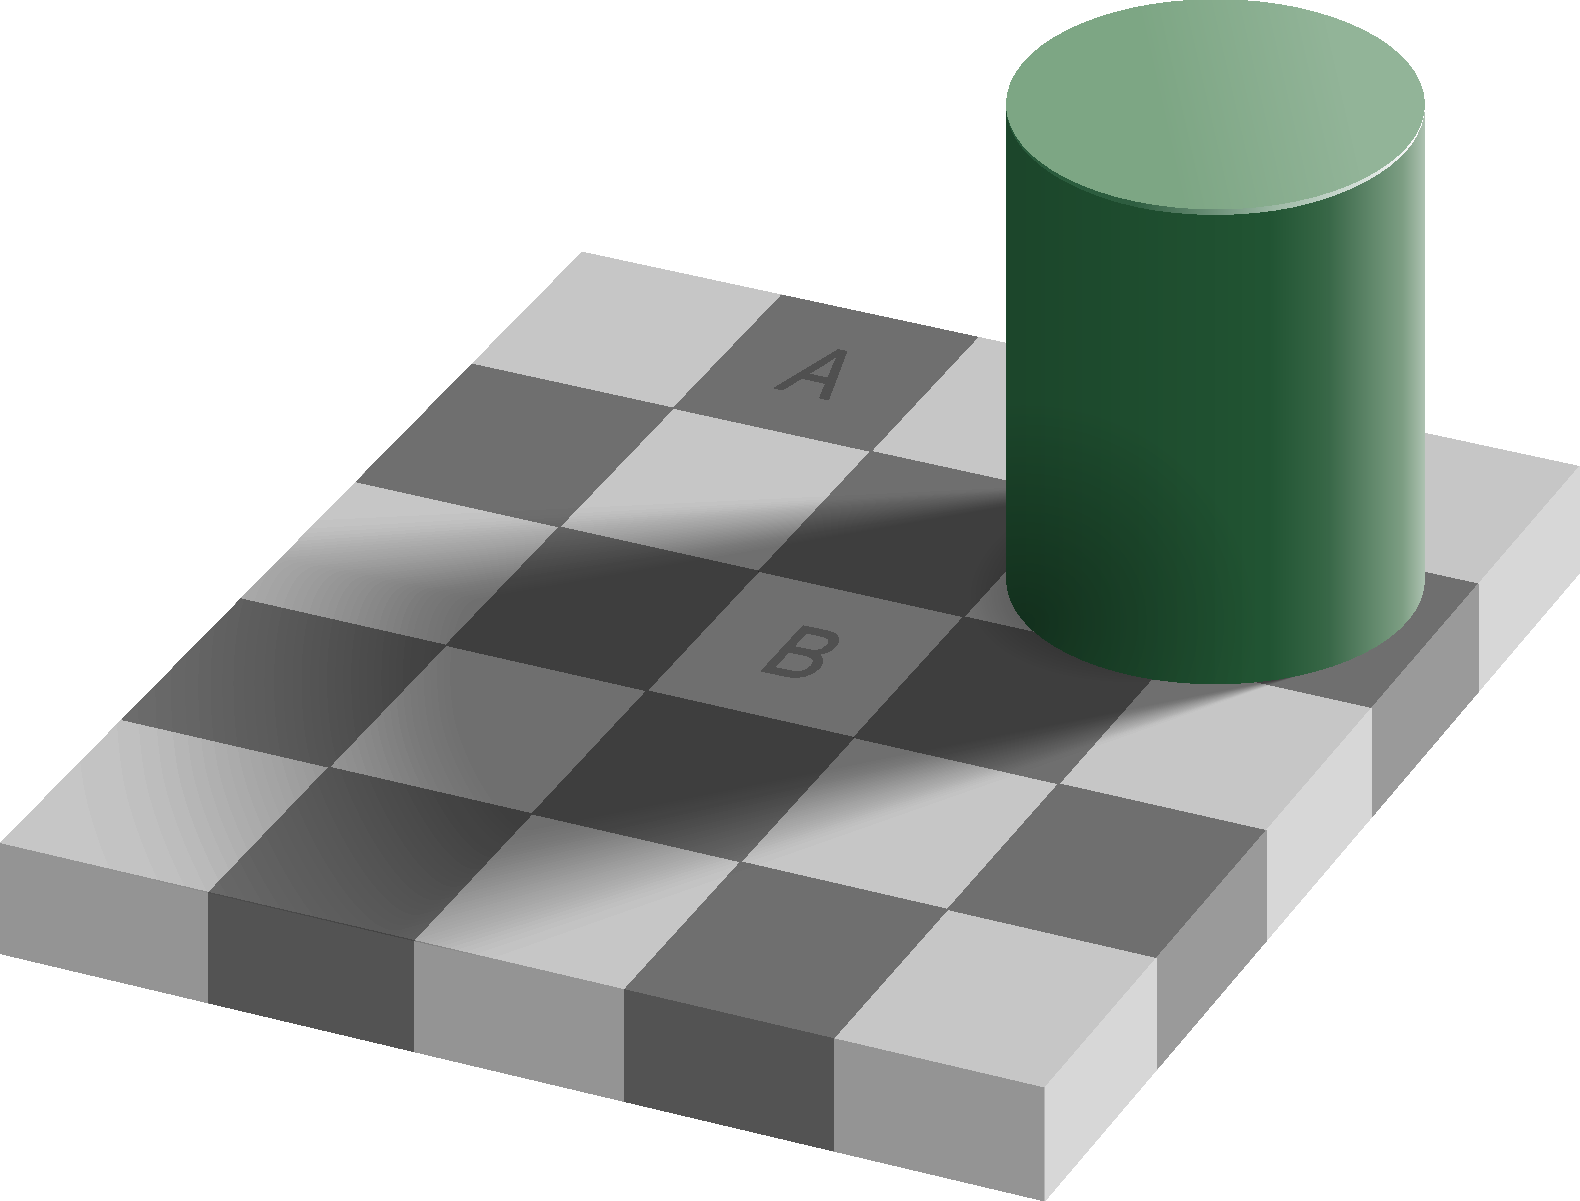
\includegraphics[width=7.4cm]{checker_shadow.pdf}};
  \begin{scope}[x={(im.south east)}, y={(im.north west)}, visible on=<2->]
    \fill[checkgray] (0.499,0.69) -- (0.547,0.69) -- (0.534,0.456) -- (0.486,0.456) -- cycle;
  \end{scope}
\end{tikzpicture}

    \end{column}
    \begin{column}{0.42\textwidth}
      \begin{itemize}
        \item Ի՞նչ գրեցիր սկզբում. A, թե B
        \item<2-> A-ն ու B-ն \textbf{նույն գույնն են}. միացնենք նույն մոխրագույնով
        \item<3-> Ուղեղը «գիտի», որ B-ն ստվերում է, ու ինքը «բացացնում» է այն
      \end{itemize}
      \onslide<3->{%
      \begin{card}[colback=butter!45!cream]
        \small Պատասխանը գիտես, բայց B-ն դեռ \textbf{բաց} է թվում։
      \end{card}}
    \end{column}
  \end{columns}
  \source{Edward H. Adelson, 1995}
\end{frame}

\begin{frame}{Ինչն է որտեղ, ու ով է դա}
  \begin{columns}[c]
    \begin{column}{0.5\textwidth}
      \centering
      \begin{tikzpicture}
        \path[use as bounding box] (-3.6,-2.4) rectangle (3.6,2.4);
        \begin{scope}[scale=0.66]
          \brainlobes{lavender!40!cream}{mint!45!cream}{peach!45!cream}{butter!80!cream}
          \fill[amRed, opacity=0.55] (3.0,-0.15) ellipse (0.3 and 0.55);
          \fill[amBlue, opacity=0.5, visible on=<2->] (1.4,1.6) ellipse (0.8 and 0.45);
          \fill[amOrange, opacity=0.8, visible on=<3->] (0.4,-1.05) ellipse (1.0 and 0.25);
          \node[wpill=amRed] at (3.6,-1.95) {տեսողական կեղև};
          \node[wpill=amBlue, visible on=<2->] at (1.6,3.05) {որտե՞ղ է};
          \node[wpill=amOrange!85!black, visible on=<3->] at (-1.5,-2.65) {ի՞նչ է, ո՞վ է};
        \end{scope}
      \end{tikzpicture}
    \end{column}
    \begin{column}{0.46\textwidth}
      \begin{itemize}
        \item Առաջնային կեղևից հեռու՝ ավելի \textbf{նեղ մասնագիտացում}
        \item<2-> Գագաթային բիլթը՝ \textbf{տարածությունը}
        \item<3-> Քունքային բլթի ստորին մասը՝ \textbf{առարկաներն ու դեմքերը}
      \end{itemize}
      \onslide<4->{%
      \begin{card}[colback=brainpink!25!cardwhite]
        \small Կա հատուկ մաս \textbf{դեմքերի} համար, ու դեմք ենք տեսնում ամենուր, նույնիսկ տոստի վրա։
      \end{card}}
    \end{column}
  \end{columns}
\end{frame}

\begin{frame}{3D՝ հարթ պատկերից}
  \begin{columns}[T]
    \begin{column}{0.5\textwidth}
      \begin{itemize}
        \item Ցանցաթաղանթը \textbf{հարթ} է, ինչպես գրատախտակը, իսկ մենք տեսնում ենք 3D
        \item<2-> Երկու աչքը տեսնում են մի քիչ \textbf{տարբեր} պատկերներ, ու ուղեղը դրանից հաշվում է խորությունը
      \end{itemize}
      \onslide<3->{%
      \begin{tryit}
        Բութ մատդ պահիր դեմքիդ առաջ ու հերթով փակիր աչքերդ. մատը «ցատկում» է։
      \end{tryit}}
    \end{column}
    \begin{column}{0.46\textwidth}
      \centering
      \onslide<4->{%
      \begin{meme}[6.3cm]{math_lady.jpg}
        \memecap[text width=4.8cm]{0.5}{0.88}{երկու հարթ պատկեր $\rightarrow$ 3D աշխարհ}
      \end{meme}}
    \end{column}
  \end{columns}
\end{frame}

\begin{frame}{Մեկ աչքով էլ է ստացվում}
  \begin{columns}[c]
    \begin{column}{0.54\textwidth}
      \centering
      % Depth cues that work with one eye: occlusion (the tree hides part of the house), texture (grass
% detail fades with distance) and lines converging into the distance (the road). Tags on slides 2-4.
\begin{tikzpicture}
  \path[use as bounding box] (-3.9,-2.15) rectangle (3.9,2.05);
  \begin{scope}
    \clip[rounded corners=3mm] (-3.8,-2.1) rectangle (3.8,2.0);
    \fill[lavender!35!cardwhite] (-3.8,0.75) rectangle (3.8,2.0);
    \fill[mint!55!cardwhite] (-3.8,-2.1) rectangle (3.8,0.75);
    % grass texture: big and sparse near, tiny and dense far
    \foreach \y/\s/\d in {-1.9/0.09/0.55, -1.45/0.07/0.45, -1.05/0.055/0.36, -0.7/0.04/0.28, -0.4/0.03/0.21, -0.15/0.022/0.16, 0.08/0.016/0.12, 0.28/0.012/0.09, 0.46/0.009/0.07}{
      \pgfmathtruncatemacro{\grassn}{7.6/\d}
      \foreach \k in {0,...,\grassn}{\fill[mintdark!70] (-3.8+\k*\d,\y) circle (\s);}}
    % road converging to the horizon
    \fill[plum!25!cardwhite] (-2.1,-2.1) -- (2.1,-2.1) -- (0.08,0.75) -- (-0.08,0.75) -- cycle;
    \draw[plum!70, line width=0.9pt] (-2.1,-2.1) -- (-0.08,0.75) (2.1,-2.1) -- (0.08,0.75);
    \foreach \a/\b in {-2.0/-1.45, -1.05/-0.68, -0.35/-0.1, 0.12/0.28, 0.42/0.52, 0.6/0.66}{
      \draw[butter!90!amOrange, line width=1.6pt] (0,\a) -- (0,\b);}
    % house, partly hidden by a tree
    \filldraw[fill=peach, draw=plum, line width=0.7pt] (1.6,0.35) rectangle (2.6,1.15);
    \filldraw[fill=plum!70, draw=plum, line width=0.7pt] (1.5,1.15) -- (2.1,1.6) -- (2.7,1.15) -- cycle;
    \node at (1.7,0.85) {\bigemoji[1.2cm]{tree}};
    % trees getting smaller along the road
    \foreach \x/\y/\h in {-2.9/-1.0/1.1, -1.85/-0.05/0.7, -1.15/0.45/0.45, -0.6/0.72/0.28}{\node at (\x,\y) {\bigemoji[\h cm]{tree}};}
  \end{scope}
  \draw[plum, line width=0.9pt, rounded corners=3mm] (-3.8,-2.1) rectangle (3.8,2.0);
  % tags
  \node[visible on=<2->, wpill=amRed] at (2.85,1.75) {1 ծածկում};
  \node[visible on=<3->, wpill=amBlue] at (-2.75,-1.8) {2 մանրամասներ};
  \node[visible on=<4->, wpill=amOrange!85!black] at (2.2,-1.8) {3 զուգահեռները հատվում են};
\end{tikzpicture}

    \end{column}
    \begin{column}{0.42\textwidth}
      \begin{itemize}
        \item Մի աչքով աշխարհը հարթ չի դառնում. ուղեղն օգտագործում է պատկերի \textbf{նշանները}
        \item<5-> Բըրնեթը ճանաչում էր միաչյա հաջողակ \textbf{ատամնաբույժի}
      \end{itemize}
      \onslide<4->{%
      \begin{scienceupdate}
        Գրքում 3-րդը կոչվում է convergence. ճիշտ տերմինը \textbf{գծային հեռանկարն} է։
      \end{scienceupdate}}
    \end{column}
  \end{columns}
\end{frame}

\begin{frame}{3D կինո}
  \centering
  % 3D cinema: two slightly shifted pictures on one screen; the glasses let each eye see only one of them;
% the brain reads the difference as depth. Reveals in 3 steps (use inside a frame).
\begin{tikzpicture}
  \path[use as bounding box] (-6.6,-1.6) rectangle (6.6,1.6);
  % screen with two overlapping pictures
  \filldraw[fill=cardwhite, draw=plum, line width=0.9pt, rounded corners=1.5mm] (-6.4,-1.1) rectangle (-3.4,1.1);
  \fill[amRed, opacity=0.55] (-5.05,0) circle (0.55);
  \fill[cyan!70!amBlue, opacity=0.55] (-4.75,0) circle (0.55);
  \node[font=\scriptsize, text=plum, align=center] at (-4.9,-1.4) {էկրանին՝ երկու պատկեր};
  % glasses
  \begin{scope}[visible on=<2->]
    \draw[warr] (-3.2,0) -- (-2.3,0);
    \filldraw[fill=amRed, fill opacity=0.5, draw=plum, line width=1pt, rounded corners=2mm] (-2.1,-0.35) rectangle (-1.2,0.35);
    \filldraw[fill=cyan!70!amBlue, fill opacity=0.5, draw=plum, line width=1pt, rounded corners=2mm] (-0.9,-0.35) rectangle (0.0,0.35);
    \draw[plum, line width=1pt] (-1.2,0.1) -- (-0.9,0.1);
    \node[font=\scriptsize, text=plum, align=center] at (-1.05,-1.4) {ակնոցը ամեն աչքին\\ թողնում է մեկը};
  \end{scope}
  % each eye gets its own picture
  \begin{scope}[visible on=<2->]
    \draw[warr] (0.2,0) -- (0.9,0);
    \node[draw=plum, line width=0.8pt, fill=cardwhite, rounded corners=1.5mm, minimum size=0.9cm] (le) at (1.5,0.55) {};
    \fill[amRed, opacity=0.55] (1.45,0.55) circle (0.3);
    \node[draw=plum, line width=0.8pt, fill=cardwhite, rounded corners=1.5mm, minimum size=0.9cm] (re) at (1.5,-0.55) {};
    \fill[cyan!70!amBlue, opacity=0.55] (1.6,-0.55) circle (0.3);
    \node[font=\scriptsize, text=plum, anchor=east] at (0.98,0.55) {\emoji{eye}};
    \node[font=\scriptsize, text=plum, anchor=east] at (0.98,-0.55) {\emoji{eye}};
  \end{scope}
  % the brain sees depth
  \begin{scope}[visible on=<3->]
    \draw[warr] (2.2,0) -- (3.0,0);
    \node at (3.75,0) {\mascot[1.5cm]{happy}};
    \node[draw=plum, line width=1pt, fill=butter, rounded corners=2mm, font=\blackfont\small, text=plum, rotate=8]
      at (5.6,0.55) {3D!};
    \node[font=\scriptsize, text=plum, align=center] at (5.2,-0.85) {տարբերությունը\\ = խորություն};
  \end{scope}
\end{tikzpicture}
\par\bigskip
  \begin{columns}[T]
    \begin{column}{0.47\textwidth}
      \small Սովորական կինոյում էլ կան խորության նշանները, բայց մենք գիտենք, որ էկրանը հարթ է։
    \end{column}
    \begin{column}{0.47\textwidth}
      \onslide<3->{\small 3D ակնոցով ամեն աչք իր պատկերն է ստանում, պատկերը «դուրս է թռչում» էկրանից, ու տոմսի համար \textbf{կրկնակի} ենք վճարում։}
    \end{column}
  \end{columns}
\end{frame}

\begin{frame}{Երկու դեմք, թե՞ ծաղկաման}
  \begin{columns}[c]
    \begin{column}{0.42\textwidth}
      \centering
      % Rubin's vase: two faces in profile looking at each other, or one vase between them.
% The vase is drawn in plum; the faces are the cream background. No reveals.
\begin{tikzpicture}[scale=0.85]
  % x = half-width of the vase (the distance from the centre line to each face's profile), top to bottom:
  % forehead, brow, eye, nose tip (narrowest), lips, chin, neck
  \fill[cardwhite] (-2.4,-2.75) rectangle (2.4,2.75);
  \fill[plum] plot[smooth, tension=0.55] coordinates {(1.55,2.6) (1.3,2.25) (0.95,1.85) (0.72,1.5) (0.86,1.18)
      (0.82,0.95) (0.5,0.62) (0.28,0.38) (0.42,0.2) (0.52,0.05) (0.4,-0.12) (0.48,-0.28) (0.38,-0.44)
      (0.58,-0.68) (0.46,-0.98) (0.42,-1.2) (0.75,-1.5) (1.05,-1.85) (1.2,-2.25) (1.25,-2.6)}
    -- (-1.25,-2.6)
    -- plot[smooth, tension=0.55] coordinates {(-1.25,-2.6) (-1.2,-2.25) (-1.05,-1.85) (-0.75,-1.5) (-0.42,-1.2)
      (-0.46,-0.98) (-0.58,-0.68) (-0.38,-0.44) (-0.48,-0.28) (-0.4,-0.12) (-0.52,0.05) (-0.42,0.2) (-0.28,0.38)
      (-0.5,0.62) (-0.82,0.95) (-0.86,1.18) (-0.72,1.5) (-0.95,1.85) (-1.3,2.25) (-1.55,2.6)} -- cycle;
  \draw[plum, line width=1pt] (-2.4,-2.75) rectangle (2.4,2.75);
\end{tikzpicture}

    \end{column}
    \begin{column}{0.54\textwidth}
      \begin{chatbox}
        Ի՞նչ տեսար \textbf{առաջինը}՝ ծաղկաման, թե՞ երկու դեմք։ Գրիր չաթում։
      \end{chatbox}
      \vspace{1mm}
      \onslide<2->{%
      \begin{itemize}
        \item Երկու պատասխանն էլ \textbf{ճիշտ} են, բայց միաժամանակ չես տեսնում
        \item Ուղեղը երկիմաստություն չի սիրում ու \textbf{ընտրում է մեկը}
        \item Բայց կարող է կարծիքը փոխել. փորձիր
      \end{itemize}}
    \end{column}
  \end{columns}
\end{frame}

\begin{frame}{Սառցաբեկորի գագաթը}
  \begin{columns}[c]
    \begin{column}{0.56\textwidth}
      \begin{card}\emoji{bread}\ \textbf{Դեմքեր}՝ քունքային կեղևի դեմքերի հատվածը\end{card}
      \begin{card}\emoji{palette}\ \textbf{Գույներ}՝ երկրորդային տեսողական կեղևը շփոթվում է ֆոնից\end{card}
      \begin{card}\emoji{question}\ \textbf{Երկիմաստություն}՝ ուղեղը ընտրում է մեկ տարբերակ\end{card}
    \end{column}
    \begin{column}{0.4\textwidth}
      \onslide<2->{%
      \begin{bookquote}
        Սա տեսողական համակարգի սառցաբեկորի գագաթն է միայն։ Իսկ խորությունը կարող ես տեսնել միայն այն պատճառով, որ տեսողական համակարգն այդքան բարդ է։
      \end{bookquote}}
    \end{column}
  \end{columns}
\end{frame}
